\chapter{Algebra Part II}

\subsection{SAT Worksheet 1F: Warm-Up Problems}

\textbf{Solve the following questions:}

\begin{multienumerate}
\mitemxx{\basic

Winifred makes \$250 a week and deposits 10\% of that into her savings account. Jenny makes \$300 a week and deposits 20\% of it into her savings. At the beginning of the month of February, Winifred's account already has \$1620 and Jenny's has \$1200. At the end of which month will they have the same amount of money in their savings account? (Assume each month to be four weeks)

\begin{enumerate}[label=(\Alph*)]
\item March
\item April
\item May
\item June
\item July
\end{enumerate}}{\medium

Steven has been working hard to try to make a specific weight bracket in wrestling that requires him to weigh somewhere between 160 and 174 pounds. If Steven's staring weight was 182 pounds and $w$ represents the amount of weight Steven loses, which inequality expresses all the possible values of $w$?

\begin{enumerate}[label=(\Alph*)]
\item $|w-22|\leq8$
\item $|w-15|\leq8/22$
\item $|w-22|\leq14$
\item $|w-167|\leq7$
\item $|w-15|\leq7$
\end{enumerate}}

\vfill
\mitemxx{\medium

Choco's Chocolate sells chocolate bars for \$3 and fudge for \$5. Max spent a total of \$27 on his recent trip to Choco's Chocolate and returned home with a bag of 7 items containing both chocolate bars and fudge. How much money did Max spend on fudge?

\begin{enumerate}[label=(\Alph*)]
\item \$9
\item \$10
\item \$12
\item \$15
\item \$20
\end{enumerate}}{\advanced

Tim's score on a test was five times the square root of Jane's and Mary's score was twice as much as Tim's. If Mary got a 90 on the test, what is the difference between Jane's and Tim's score?

\begin{enumerate}[label=(\Alph*)]
\item 36
\item 45
\item 9
\item 81
\item 26
\end{enumerate}}
\end{multienumerate}

\newpage
\section{Patters and Sequences}

A remainder is the amount left over after \longline. For example, six will divide into 19 three times with a remainder of \longline.
We can usually use one of two strategies to solve these types of problems.

\vfill
\textbf{Strategy \#1:} If a remainder problem contains a variable problem, then we can

\longline that fits the parameters and then use this number to solve for what the problem is asking. 

\bigskip
For example: When 2m is a divided by 4, the remainder is 5. What will the remainder be when $3m$ is divided by 10?

\vfill
\textbf{Strategy \#2:} Then you need to come up with \longline and solve for the \longline in order to solve. 
For example, When 48 is divided by a positive integer $n$, the remainder is 4. How many values of $n$ are possible?

\vfill
We are also going to use a strategy similar to Strategy \#2 in order to solve problems that repeat numbers, symbols, etc. by using divisibility rules. We are particularly interested in the  \longline.

\bigskip
For example, A fashionista is laying out her colored scarves. She first lays down 2 red scarves, then 3 blue scarves, then 1 green scarf, then 2 orange scarves, then 1 pink scarf. She repeats this pattern until she has laid out all 1,000 scarves. What color is the 782\textsuperscript{nd} scarf?

\begin{enumerate}[label=(\Alph*)]
\item red
\item blue
\item green
\item orange
\item pink
\end{enumerate}

\begin{enumerate}
\item Start by writing \longline iterations of the pattern on top of each other:
\vfill\item \longline the end of each line
\vfill\item You will see that you are counting up by \longline occurring in the first line
\vfill\item Divide the \longline by the \longline.

Find the \longline.
\vfill\item Start at the beginning of the pattern. Count each unique item in the pattern until you reach the same number as the \longline. This item in the pattern is the \longline.
\end{enumerate}

Example \#2: There are 5 ducks in a row behind the mother ducks, Ariel, Boston, Carl, Devin, and Edward. Every day, the ducks take a turn swimming behind the mother so it is Ariel's turn, then Boston's turn, then Carl's turn, then Devin's turn, then Edward's turn. If Boston swims behind his mother on the first day, who will be swimming behind the mother on the 42\textsuperscript{nd} day?

\begin{enumerate}[label=(\Alph*)]
\item Ariel
\item Boston
\item Carl
\item Devin
\item Edward
\end{enumerate}

\vfill
Example \#3: Every day, Steven runs one errand or completes one chore. On the first day, he goes to the grocery store. On the next day, he goes to the laundry mat, and on the next day, he goes to the pharmacy. On the next day, Steven goes to the car mechanic, and on the next day, he cleans the house. After this, he repeats his chore list (so the day after cleaning the house, he goes to the grocery store). One day that he went to the car mechanic, he went to the movies immediately afterwards. Which of the following could be the number of days he did chores prior to the day that he decided to go to the movies? \textbf{[Note: In previous problems, it has given you the total number and wants you to find the unique item. This problem gives you the unique item, that he goes to the movies, and wants you to use divisibility rules to find the total number. You can use steps \#1-5 above, but you need to reverse them.]}

\begin{enumerate}[label=(\Alph*)]
\item 30
\item 74
\item 143	%so much was wrong with this question but it should be fixed now
\item 271
\item 362
\end{enumerate}

\vfill
Example \#4: $6, 11, 16, 21, \ldots$

\bigskip
Each term in the sequence after the first term is 5 more than the term before it. The 45\textsuperscript{th} term than the 37\textsuperscript{th} term? \textbf{The challenge is to solve this without solving for the 37\textsuperscript{th} and the 45\textsuperscript{th} term.}

\begin{enumerate}[label=(\Alph*)]
\item 18
\item 25
\item 37
\item 38
\item 40
\end{enumerate}

\vfill
We will use the idea of writing out the possible items to solve problems that ask about the minimum number of items selected in order to guarantee some situation. 

\bigskip
For example, there are 144 marbles in a box. There are 24 marbles of each of the following colors: red, blue, green, white, black, and gray. Tom randomly selects marbles from the box.

\begin{enumerate}[label=\alph*)]
\item What is the minimum number of marbles Tom needs to select in order to guarantee that he gets at least two marbles of the same color? 

\bigskip
To solve this, we need to think of the \longline. In this scenario, he selects \longline before he selects a second marble of any color. 


\vfill
\item What is the minimum number of marbles Tom needs to select in order to guarantee that he gets at least two marbles of the same color?
\end{enumerate}

\vfill
\newpage
\subsection{SAT Worksheet 2F: 4 Questions, 5 Minutes}

\begin{multienumerate}
\mitemxx{\basic

When $k$ is divided by 10, the remainder is 5. $k$ could have which of the following as factors?

\begin{enumerate}[label=\Roman*.]
\item 2
\item 3
\item 5
\end{enumerate}

\begin{enumerate}[label=(\Alph*)]
\item I only
\item II only
\item I and II only
\item II and III only
\item I, II, and III
\end{enumerate}}{\basic

$7.03615036150361\ldots$

The decimal number above continues to repeat to the 100\textsuperscript{th} digit to the right of the decimal point. What is the 20\textsuperscript{th} digit to the right of the decimal place?

\begin{enumerate}[label=(\Alph*)]
\item 0
\item 3
\item 6
\item 1
\item 5
\end{enumerate}}

\vfill
\mitemxx{\medium

$7.036150361503615\ldots$

The decimal number above continues to repeat until the 100\textsuperscript{th} digit to the right of the decimal point. What is the product of values from the 90\textsuperscript{th} digit to the 92\textsuperscript{nd} digit to the right of the decimal place?}{\advanced

$1.566566665\ldots$

In the number above, the decimal number contains only 5's and 6's. The first 5 is followed by two 6's, the second 5 is followed by four 6's, and the $n$\textsuperscript{th} 5 is followed by $2n$ number of 6's. How many 6's are between the 47\textsuperscript{th} number 5 and the 51\textsuperscript{st} number 5?}
\end{multienumerate}

\vfill
\newpage
\section{Probability}

In general, probability of an event is occurring is defined as:

\vfill
The most difficult type of probability questions are when multiple events are occurring because you must take into account the wording of the question to give you a clue as to whether the events are happening together or separately and also if the items are getting replaced or not (as this will affect the denominator when you are solving the problem). 
Probability is a number between \shortline and \shortline. \shortline represents the sum of all of the events that could happen. For example, on a fair two-sided coin, the options from one coin flip are getting a tails or a head (and nothing else). The probability of getting the tail side is ½ and the probability of getting the head side is $1/2$ and$1/2 + 1/2 =1$.

\vfill
If you want to know the probability of an event not happening, you will need to find the probability of it happening and subtract this probability from \shortline. This is called the \longline.

\vfill
\longline events are when the results of the first event affects the probability of the second event occurring or not occurring.

\vfill
\longline events are when the results of the first event affects the probability of the second event occurring or not occurring.

\vfill
If you want to know the probability of two independent events happening, then

\longline the probabilities. For example, you would use this method when you select a ball from a jar, put it back in the jar, and then choose another ball (called choosing with replacement).

\vfill
If you want to know the probability of two dependent events happening, then you will need to \longline the probability of the second event based on the first event happening. For example, you would use this method when you select a ball from a jar, and then choose another ball without putting the first ball back (called choosing without replacement).  If the probability of choosing a green ball is 7/10 and you want to know the probability of choosing two green balls in a row without replacement, then you calculate the probability of the first ball being green, 7/10, and the second ball being green with the first green ball removed, which is $(7 - 1)/(10 - 1) = 6/9$. Therefore, the probability of getting two green balls in a row without replacement of the first ball would be $7/10 \cdot 6/9 = 42/90$.

\vfill
If you want to know the probability of neither happening, you will need to find the probability of either happening and subtract this probability from \shortline. This is called the \longline.

\vfill
\newpage
We will now use one example and see how many ways a problem can be asked. In each case, there are 10 red balls and 12 blue balls in Jar $A$ and 3 red balls and 9 blue balls in Jar $B$. Show your work when solving for each problem so that you can see the differences between the words and problem-solving steps for it. 

\begin{enumerate}[label=\alph*)]
\item A person picks one ball from Jar A, records the color, puts it back in the jar and then picks a ball from Jar B. What is the probability that the first ball is red or the second ball is blue?
\vfill\item A person picks one ball from Jar A, records the color, and picks a ball from Jar B. What is the probability that the first ball is red and the second ball is blue?
\vfill\item What is the difference in wording between a) and b)? How does this account for different approaches that you need to use to solve the two problems?
\vfill\item A person picks one ball from Jar A, records the color, and picks another ball from Jar A without putting the first ball back in the jar. What is the probability that both balls selected are red?
\vfill\item A person picks one ball from Jar A, records the color, and picks another ball from Jar A without putting the first ball back in the jar What is the probability that both balls selected are the same color?
\vfill\item What is the difference in wording between d) and e)? How does this account for different approaches that you need to use to solve the two problems?
\vfill\item g)	A person picks one ball from Jar A, records the color, replaces the first ball and picks another ball from Jar A. What is the probability that both balls selected are red?
\vfill\item What is the difference in wording between d) and g)? How does this account for different approaches that you need to use to solve the two problems?
\end{enumerate}

\vfill
\newpage
\subsection{SAT Worksheet 3F (Basic): 6 Questions, 8 Minutes}

\begin{multienumerate}
\mitemxx{1.	Ms. Ziggy has a jar with 6 red marbles, 4 blue marbles, and 5 green marbles. If a student removes two marbles, one at a time, what is the probability that a student will randomly pick 2 red marbles in a row?

\begin{enumerate}[label=(\Alph*)]
\item 1/7
\item 2/7
\item 2/5
\item 3/5
\item 2/3
\end{enumerate}}{Sally has 3 pairs of color shoe laces, 2 pairs of shoes, and 4 pairs of color socks. How many combinations of laces, shoes, and socks does Sally have?

\begin{enumerate}[label=(\Alph*)]
\item 9
\item 10
\item 11
\item 12
\item 24
\end{enumerate}}

\vfill
\mitemxx{

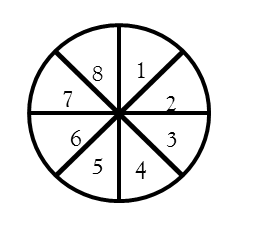
\includegraphics{54}

What is the probability of landing on a prime number on the spinner above?

\begin{enumerate}[label=(\Alph*)]
\item 1/4
\item 3/8
\item 1/2
\item 5/8
\item 3/4
\end{enumerate}
}{What is the missing term in the following sequence?

$64, -32, 16, \shortline, 4, -2, 1$

\begin{enumerate}[label=(\Alph*)]
\item 9
\item 8
\item -8
\item 12
\item -12
\end{enumerate}}

\vfill
\mitemxx{Accounts at General Bank Savings ATMs require four digits pins such that no digit is repeated. How many possible combinations of pins are possible?

\begin{enumerate}[label=(\Alph*)]
\item 1920
\item 3024
\item 5040
\item 6561
\item 10,000
\end{enumerate}}{If there are 4 queens and 4 kings in a standard deck of 52 cards, what are the odds of choosing a queen or a king?

\begin{enumerate}[label=(\Alph*)]
\item 1/13
\item 2/13
\item 4/13
\item 1/169
\item 2/169
\end{enumerate}}
\end{multienumerate}

\newpage
\subsection{SAT Worksheet 4F (Medium): 6 Questions, 9 Minutes}

\begin{multienumerate}
\mitemxx{The sum of the angles of an n-sided regular polygon can be found by adding 180 to the sum of the angles of a regular polygon of one less side. If the sum of the angles of a square is 360, what is the value of one angle of a 10-sided regular polygon?

\begin{enumerate}[label=(\Alph*)]
\item 72
\item 80
\item 120
\item 144
\item 162
\end{enumerate}}{A hat contains the numbers from 1 to 20. What is the probability of picking out a number that is not a perfect square?

\begin{enumerate}[label=(\Alph*)]
\item 0.15
\item 0.20
\item 0.75
\item 0.80
\item 0.85
\end{enumerate}}

\vfill
\mitemxx{

\medskip
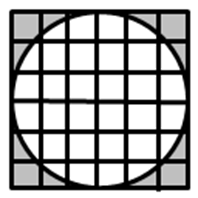
\includegraphics{55}

A circle of radius 3 units is inscribed in a square. If a dart that occupies 1 square unit is tossed at the board, state the odds of the dart landing within the circle to the nearest hundredth.}{What is the smallest possible three digit integer whose prime factors are non-repeating?

\begin{enumerate}[label=(\Alph*)]
\item 120
\item 144
\item 210
\item 330
\item 378
\end{enumerate}}

\vfill
\mitemxx{If $n$ is a positive integer, which of the following expressions does not necessarily have a factor of 3?

\begin{enumerate}[label=(\Alph*)]
\item $3n+3$
\item $6n$
\item $6(n-1)$
\item $3^n$
\item $n^3$
\end{enumerate}}{The largest number of a set of four consecutive integers is the smallest number of a different set of four consecutive integers. What is the difference between the smallest number of the first set to the largest number of the second set?

\begin{enumerate}[label=(\Alph*)]
\item 4
\item 5
\item 6
\item 7
\item 8
\end{enumerate}}
\end{multienumerate}

\newpage
\subsection{SAT Worksheet 5F (Advanced): 6 Questions, 10 Minutes}

\begin{multienumerate}
\mitemxx{If the first term of a sequence is $n$, and each subsequent term is found by adding 1 more than the previous term, which expression represents the sixth term?

\begin{enumerate}[label=(\Alph*)]
\item $n+5$
\item $6n$
\item $6n+5$
\item $6n+15$
\item $6n+21$
\end{enumerate}}{If $n$ is a positive integer, which of the following expressions cannot represent a prime number?
\begin{enumerate}[label=(\Alph*)]
\item $n^2-1$
\item $n+1$
\item $2n+1$
\item $2(n-1)+6$
\item $2^n-1$
\end{enumerate}}

\vfill
\mitemxx{For which of the following numbers is the sum of its factors, not including the number itself?

\begin{enumerate}[label=(\Alph*)]
\item 4
\item 10
\item 12
\item 24
\item 28
\end{enumerate}}{Which of the following expressions does not represent the sum of four consecutive integers?

\begin{enumerate}[label=(\Alph*)]
\item $4n-1$
\item $4n$
\item $4n+2$
\item $4n+3$
\item $4n+4$
\end{enumerate}}

\vfill
\mitemxx{A number, $n$, is divided by 3 and has a remainder of 1. When the quotient is divided by 3, the remainder is 2. For any positive integer $k$, which of the following expressions represents all possible values of $n$?

\begin{enumerate}[label=(\Alph*)]
\item $3k-1$
\item $3k+2$
\item $9k+7$
\item $9k$
\item $9k-1$
\end{enumerate}}{Let $n$ be a number with $d$ factors. If $d$ is an odd number, which of the following must be true?


\begin{enumerate}[label=\Roman*.]
\item $n/d$ must also be odd
\item $n$ is a perfect square
\item $n-d$ must be odd
\end{enumerate}

\begin{enumerate}[label=(\Alph*)]
\item I only
\item II only
\item III only
\item I and II
\item I, II, and III
\end{enumerate}}
\end{multienumerate}